\documentclass{article}
\usepackage[paperwidth=13.5cm,paperheight=7.2cm,margin=0.15cm]{geometry}
\usepackage{amsmath,amssymb}
\usepackage{xcolor}
\usepackage{tikz}
\usetikzlibrary{arrows.meta,positioning,calc,fit,shapes.geometric,backgrounds}

\begin{document}
\pagestyle{empty}
\centering

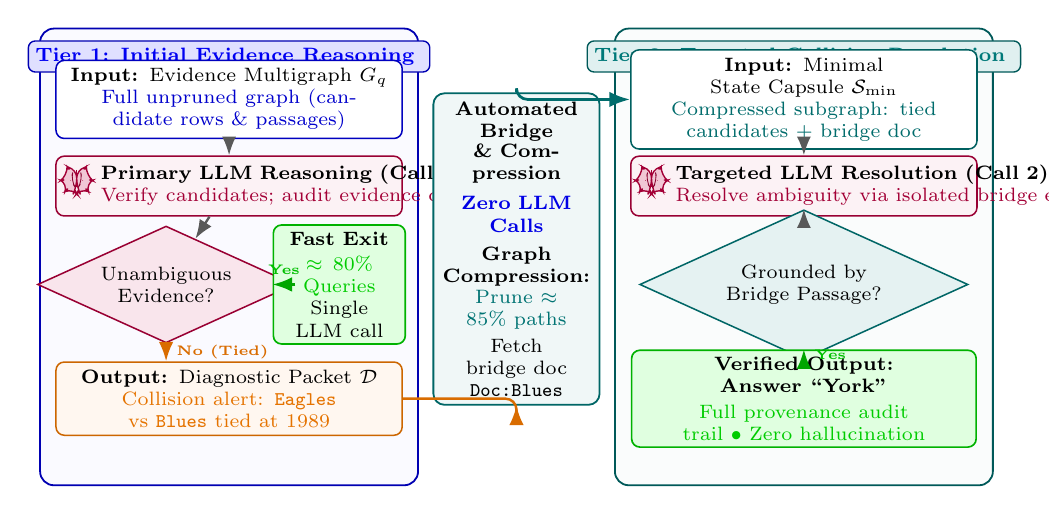
\begin{tikzpicture}[
  >=Latex,
  font=\sffamily\scriptsize,
  % Panels
  col_panel/.style={draw=#1!70!black, fill=#1!2!white, rounded corners=5pt, line width=0.65pt},
  col_hdr/.style={fill=#1!12, draw=#1!70!black, line width=0.5pt, rounded corners=2.5pt, font=\bfseries\scriptsize, text=#1!95!black, inner sep=2.5pt, align=center},
  % Flowchart Nodes
  fc_box/.style={draw=#1!75!black, fill=white, rounded corners=3pt, line width=0.55pt, inner sep=2.8pt, align=center, font=\scriptsize},
  fc_proc/.style={draw=purple!80!black, fill=purple!5, rounded corners=3pt, line width=0.55pt, inner sep=2.8pt, align=center, font=\scriptsize},
  fc_dec/.style={diamond, aspect=2.2, draw=#1!80!black, fill=#1!10, line width=0.55pt, inner sep=1.2pt, align=center, font=\scriptsize},
  fc_exit/.style={draw=green!70!black, fill=green!12, rounded corners=3pt, line width=0.6pt, inner sep=2.5pt, align=center, font=\scriptsize},
  fc_out/.style={draw=orange!80!black, fill=orange!6, rounded corners=3pt, line width=0.55pt, inner sep=2.8pt, align=center, font=\scriptsize},
  % Bridge Box
  bridge_box/.style={draw=teal!80!black, fill=teal!6, rounded corners=4pt, line width=0.65pt, inner sep=3pt, align=center, font=\scriptsize},
  % Arrows
  arr/.style={->, line width=0.85pt, draw=gray!70!black},
  arr_green/.style={->, line width=0.9pt, draw=green!65!black},
  arr_orange/.style={->, line width=0.9pt, draw=orange!85!black},
  arr_bridge/.style={->, line width=1.0pt, draw=teal!85!black}
]

% Brain icon pic
\tikzset{
  brain_icon/.pic={
    \begin{scope}[scale=0.17]
      \draw[fill=purple!22, draw=purple!85!black, line width=0.5pt]
        (0, 0.72) 
        .. controls (-0.35, 0.82) and (-0.72, 0.62) .. (-0.72, 0.28)
        .. controls (-0.92, 0.12) and (-0.92, -0.22) .. (-0.68, -0.34)
        .. controls (-0.76, -0.58) and (-0.52, -0.78) .. (-0.28, -0.68)
        .. controls (-0.18, -0.82) and (-0.05, -0.68) .. (0, -0.58)
        -- cycle;
      \draw[fill=purple!22, draw=purple!85!black, line width=0.5pt]
        (0, 0.72) 
        .. controls (0.35, 0.82) and (0.72, 0.62) .. (0.72, 0.28)
        .. controls (0.92, 0.12) and (0.92, -0.22) .. (0.68, -0.34)
        .. controls (0.76, -0.58) and (0.52, -0.78) .. (0.28, -0.68)
        .. controls (0.18, -0.82) and (0.05, -0.68) .. (0, -0.58)
        -- cycle;
      \draw[purple!85!black, line width=0.5pt] (0, 0.70) -- (0, -0.56);
      \fill[purple!85!black] (-0.35, 0.3) circle (0.75pt);
      \fill[purple!85!black] (-0.45, -0.1) circle (0.75pt);
      \fill[purple!85!black] (-0.25, -0.4) circle (0.75pt);
      \draw[purple!70!black, line width=0.3pt] (-0.35, 0.3) -- (-0.45, -0.1) -- (-0.25, -0.4);
      \fill[purple!85!black] (0.35, 0.3) circle (0.75pt);
      \fill[purple!85!black] (0.45, -0.1) circle (0.75pt);
      \fill[purple!85!black] (0.25, -0.4) circle (0.75pt);
      \draw[purple!70!black, line width=0.3pt] (0.35, 0.3) -- (0.45, -0.1) -- (0.25, -0.4);
    \end{scope}
  }
}

% -------------------------------------------------------------
% GEOMETRY:
% Width: 12.2 cm
% Col 1: Center X = 2.45cm, Width = 4.8cm (X from 0.05 to 4.85)
% Center Gap: X from 4.85 to 7.35 (Width = 2.5cm, Center X = 6.1cm)
% Col 2: Center X = 9.75cm, Width = 4.8cm (X from 7.35 to 12.15)
% Height: 5.8cm (Y from +2.9 to -2.9)
% -------------------------------------------------------------

% -------------------------
% COLUMN 1: TIER 1 ALGORITHM
% -------------------------
\node[col_panel=blue, minimum width=4.8cm, minimum height=5.8cm] (c1) at (2.45, 0) {};
\node[col_hdr=blue, minimum width=4.5cm, anchor=north] (t1_hdr) at ([yshift=-1.6mm]c1.north) {
  Tier 1: Initial Evidence Reasoning
};

% T1 Step 1: Input Box
\node[fc_box=blue, text width=4.2cm] (t1_in) at (2.45, 2.0) {
  \textbf{Input:} Evidence Multigraph $G_q$\\
  \textcolor{blue!80!black}{Full unpruned graph (candidate rows \& passages)}
};

% T1 Step 2: Primary LLM Reasoning
\node[fc_proc, text width=4.2cm] (t1_proc) at (2.45, 0.90) {
  \begin{tabular}{@{}c@{\hspace{4pt}}l@{}}
    \tikz{\pic {brain_icon};} &
    \begin{tabular}{@{}l@{}}
      \textbf{Primary LLM Reasoning (Call 1)}\\
      \textcolor{purple!85!black}{Verify candidates; audit evidence clarity}
    \end{tabular}
  \end{tabular}
};

% T1 Step 3: Decision Diamond
\node[fc_dec=purple, text width=2.0cm] (t1_dec) at (1.65, -0.35) {
  Unambiguous\\Evidence?
};

% T1 Exit: Fast Exit
\node[fc_exit, text width=1.5cm] (t1_exit) at (3.85, -0.35) {
  \textbf{Fast Exit}\\[0.4mm]
  \textcolor{green!80!black}{$\approx 80\%$ Queries}\\
  Single LLM call
};

% T1 Step 4: Output Diagnostic Packet
\node[fc_out, text width=4.2cm] (t1_out) at (2.45, -1.80) {
  \textbf{Output:} Diagnostic Packet $\mathcal{D}$\\
  \textcolor{orange!90!black}{Collision alert: \texttt{Eagles} vs \texttt{Blues} tied at 1989}
};

% Connectors in Tier 1
\draw[arr] (t1_in) -- (t1_proc);
\draw[arr] (t1_proc) -- (t1_dec);
\draw[arr_green] (t1_dec.east) -- node[above, font=\bfseries\tiny, text=green!75!black] {Yes} (t1_exit.west);
\draw[arr_orange] (t1_dec.south) -- node[right, font=\bfseries\tiny, text=orange!85!black] {No (Tied)} (t1_dec.south |- t1_out.north);


% -------------------------
% COLUMN 2: TIER 2 ALGORITHM
% -------------------------
\node[col_panel=teal, minimum width=4.8cm, minimum height=5.8cm] (c2) at (9.75, 0) {};
\node[col_hdr=teal, minimum width=4.5cm, anchor=north] (t2_hdr) at ([yshift=-1.6mm]c2.north) {
  Tier 2: Targeted Collision Resolution
};

% T2 Step 1: Input Box
\node[fc_box=teal, text width=4.2cm] (t2_in) at (9.75, 2.0) {
  \textbf{Input:} Minimal State Capsule $\mathcal{S}_{\mathrm{min}}$\\
  \textcolor{teal!85!black}{Compressed subgraph: tied candidates + bridge doc}
};

% T2 Step 2: Targeted LLM Call
\node[fc_proc, text width=4.2cm] (t2_proc) at (9.75, 0.90) {
  \begin{tabular}{@{}c@{\hspace{4pt}}l@{}}
    \tikz{\pic {brain_icon};} &
    \begin{tabular}{@{}l@{}}
      \textbf{Targeted LLM Resolution (Call 2)}\\
      \textcolor{purple!85!black}{Resolve ambiguity via isolated bridge evidence}
    \end{tabular}
  \end{tabular}
};

% T2 Step 3: Decision Diamond
\node[fc_dec=teal, text width=2.8cm] (t2_dec) at (9.75, -0.35) {
  Grounded by\\Bridge Passage?
};

% T2 Step 4: Final Verified Answer
\node[fc_exit, text width=4.2cm] (t2_out) at (9.75, -1.80) {
  \textbf{Verified Output: Answer ``York''}\\[0.4mm]
  \textcolor{green!80!black}{Full provenance audit trail $\bullet$ Zero hallucination}
};

% Connectors in Tier 2
\draw[arr] (t2_in) -- (t2_proc);
\draw[arr] (t2_proc) -- (t2_dec);
\draw[arr_green] (t2_dec.south) -- node[right, font=\bfseries\tiny, text=green!75!black] {Yes} (t2_out.north);


% -------------------------------------------------------------
% CENTER CONNECTOR: BRIDGE SEARCH & GRAPH COMPRESSION
% -------------------------------------------------------------
\node[bridge_box, text width=1.9cm] (bridge) at (6.1, 0.1) {
  \textbf{Automated Bridge}\\[-0.2mm]
  \textbf{\& Compression}\\[1.0mm]
  \textcolor{blue!90!black}{\textbf{Zero LLM Calls}}\\[0.8mm]
  \textbf{Graph Compression:}\\[-0.2mm]
  \textcolor{teal!90!black}{Prune $\approx 85\%$ paths}\\[0.6mm]
  Fetch bridge doc\\
  \texttt{Doc:Blues}
};

% Inter-tier connecting flow
\draw[arr_orange, rounded corners=4pt] (t1_out.east) -- (6.1, -1.80) -- (bridge.south);
\draw[arr_bridge, rounded corners=4pt] (bridge.north) -- (6.1, 2.0) -- (t2_in.west);

\end{tikzpicture}
\end{document}
